
%\usepackage{algorithmic}
%\usepackage{algorithm}
%\usepackage{program}
%\usepackage{programs}



\section{Preprocessing w bazie danych}

W bazie danych wyliczone zostają informacje potrzebne do późniejszego utworzenia macierzy używanych w algorytmach Adapted PageRank i Social PageRank. Algorytmy te przy każdym przebiegu korzystają z tych samych macierzy, obliczanie ich przy każdej iteracji wymagałoby zbyt dużego nakładu czasu. Dane te są wyliczane w dwóch częściach. Na początku wyliczane są w bazie danych i zapisywane w pomocniczych tabelach. Następnie zapisywane są one do do struktury i serializowane w oddzielnych plikach. Pliki te są później używane do tworzenia macierzy.

Informacje te zostaną zapisane w tabeli USERTAGDOC w polu how\_much i w tabelach TAG\_USR i TAG\_DOC. Wyliczenie tych informacji pozwoli później na szybszy dostęp do nich.

Czas wykonania preprocessingu w bazie danych jest różny. Jak widać w tabeli poniżej (\ref{tab:czas_tabele}) najwięcej czasu trwało tworzenie tabeli TAG\_USR i powstało w niej najwięcej nowych rekordów. Wykonywanie tych obliczeń przy każdej iteracji algorytmu spowodowałoby znacznie zwiększenie czasu działania aplikacji.

\begin{table}[hbp]
  \centering
    \begin{tabular}{ | c | p{3cm}| p{3cm} | }
    \hline
    Tabela & czas wykonania polecenia & ilość powstałych rekordów  \\ 
    \hline
    TAG\_USR & FIXME & FIXME   \\ 
    \hline
    TAG\_DOC & ok 3h &  FIXME  \\ 
    \hline
    USERTAGDOC & FIXME  & FIXME  \\ 
    \hline
    \end{tabular}
     \caption{Czas wykonania wypełnienia odpowiednich tabel w bazie danych !FIXME!}
    \label{tab:czas_tabele}
   
\end{table}


Poniżej znajdują się listingi zapytań SQL obliczających pola tabeli USERTAGDOC \ref{sql_usrtagdoc} i wypełniające tabele TAG\_USR (\ref{sql_tag_doc}) i TAG\_DOC (\ref{sql_tag_usr}). 


\lstset{language=SQL}   
\begin{lstlisting}[frame=lines, caption={Skrypt dodający dane do tabeli tag\_doc}, label={sql_tag_doc}]
insert into tag_doc (doc_id, tag_id, how_much) 
select d.new_id, tag.new_id, count(utd.user_id)
from 
tag, 
usertagdoc_tag as utd_t,
usertagdoc as utd, document as d
where
d.id = utd.doc_id 
and utd_t.usertagdoc_id = utd.id 
and utd_t.tags_id = tag.id
group by utd.doc_id, tag.id;

\end{lstlisting}

\begin{lstlisting}[frame=lines, caption={Skrypt dodający dane do tabeli tag\_usr}, label={sql_tag_usr}]]
insert into tag_usr (tag_id, user_id, how_much)
select utd.user_id, tag.new_id, count(utd.doc_id)
from
tag,
usertagdoc_tag as utd_t,
usertagdoc as utd
where
utd_t.usertagdoc_id = utd.id and
utd_t.tags_id = tag.id
\end{lstlisting}

\begin{lstlisting}[frame=lines, caption={Skrypt updatujący pole how\_much w tabeli usertagdoc}, label={sql_usrtagdoc}] ]
update usertagdoc utd
set how_much = (select count(distinct tags.tags_id)
from usertagdoc_tag tags
where utd.id = tags.usertagdoc_id);
\end{lstlisting}


\subsection{Preprocessing: zapis do plików}
Po wyliczeniu w bazie danych pomocniczych tabel, wyniki są pobierane przez program, a następnie zapisywane do pliku. Ponieważ pamięć maszyny ogranicza wielkość macierzy na której jesteśmy w stanie operować, tworzone pliki zawierają tylko wyznaczoną ilość wierszy. Ilość wierszy macierzy zapisanych w pliku jest konfigurowalna i zależna od przydzielonej pamięci aplikacji.


W czasie działania algorytmów wymagane są również traspozycje wybranych macierzy. Ponieważ ograniczenia pamięciowe uniemożliwiają obrócenie macierzy w pamięci, w plikach zapisane zostaną również traspozycje macierzy.


\begin{figure}[htb]
\centering
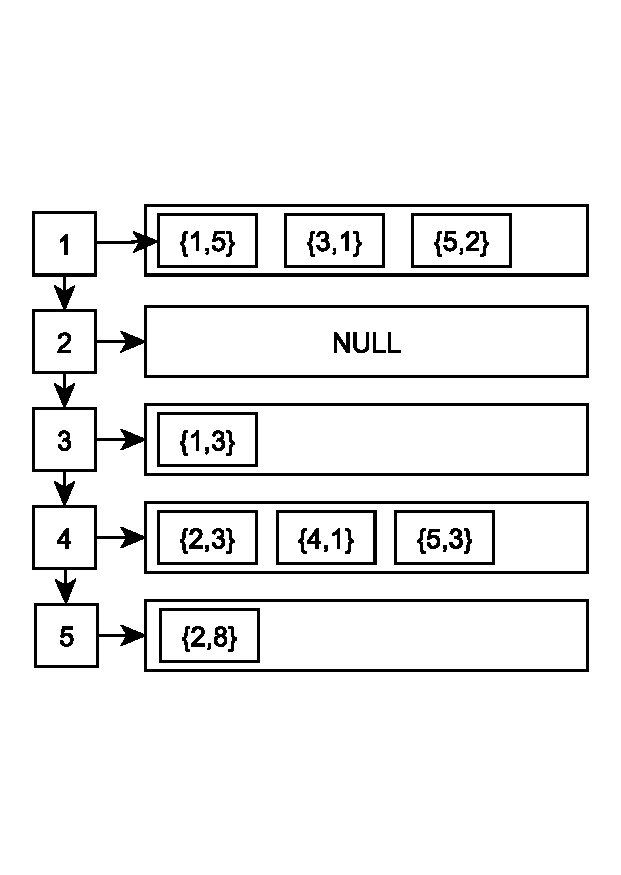
\includegraphics[width=0.5\textwidth, trim = 0mm 33mm 0mm 33mm, clip]{file_processing.pdf}
\caption{Struktura zapisana w pliku}
\label{fig:preprocessing_fig}
\end{figure}

Wynikiem działania tej części preprocesingu jest struktura będąca HashMapą. Zawierająca ona w komórce $i$ listę wszystkich niezerowych elementów znajdujących się w i-tym wierszu macierzy wraz z ich wartościami. Figura \ref{fig:preprocessing_fig} pokazuje fragment macierzy, który zostanie zapisany do pliku. Poniżej znajduje sie macierz $M_{5,5}$, która powstanie ze struktury przedstawionej na \ref{fig:preprocessing_fig}


\[
 M_{5,5} =
 \begin{pmatrix}
5 & 0 & 1 & 0 & 2\\
0 & 0 & 0 & 0 & 0\\
3 & 0 & 0 & 0 & 0\\
0 & 3 & 0 & 1 & 3\\
0 & 8 & 0 & 0 & 0\\

 \end{pmatrix}
\]


\subsection{Inne metody przyśpieszenia wykonywanych preprocesingów}

Jednym z głównym problemów jest to, że w czasie wykonywania wymienionych powyżej procedur, tabele USER, TAG i DOCUMENT są zablokowane na zmiany. W działającej aplikacji byłoby to poważnym problemem.  

Można poradzić sobie z tym problemem poprzez posiadanie kopi bazy danych i uzupełnianie obydwu jednocześnie. Dzięki czemu operacje wymagające dużej ilości czasu, mogłyby być wykonane na innej bazie. Po dokonaniu wszystkich obliczeń wymagane jest zsynchronizowanie obydwu baz danych.

Inną możliwością jest zrównoleglenie wykonywanych obliczeń. Możliwe jest na przykład: podzielenie obliczenia tabel TAG\_DOC, TAG\_USER i USERTAGDOC na różne maszyny. Dodatkową możliwością jest podzielenie samych tabel na różne procesy. Na przykład wyliczanie tabeli TAG\_DOC można podzielić na niezależne procesy ze względu na pole ID obiektów z tabeli TAG. Analogicznie można przeprowadzić taki podział dla innych tabel.

Kolejną możliwością są zmiany danych w tabelach TAG\_DOC, TAG\_USER i USERTAGDOC w czasie kiedy dodawane są nowe rekordy do tabel USER, DOCUMENT i TAG. Wyeliminowało by to potrzebę wykonywania opisane powyżej preprocesingu, ale stanowiło by problem przy tworzeniu macierzy. Tworzenie macierzy (dokładnie: plików z których następnie tworzona jest macierz) jest czasochłonne i wymaga zatrzymania zmian dokonywanych na tabelach TAG\_DOC, TAG\_USER i USERTAGDOC. Problem ten dałoby się rozwiązać przez np: posiadanie kopi wymienionych wcześniej tabel. Synchronizacja kopi tabeli i głównej tabeli nie zajmowała by aż tak wiele czasu. Pomysł ten spowodował by jeszcze jeden potencjalnie groźny problem. Ilość operacji, które trzeba by wykonać w czasie gdy dodawane są nowe rekordy do tabel, znacznie by się zwiększyła. Mogłoby to spowodować większą awaryjność np: problemy z transakcjami.











